\documentclass{article}

%% Denote paragraphs with vertical space rather than indenting (not critical)
\usepackage{parskip}

%% Support for URL in introductory text (not needed for main example)
\usepackage{url}

%% *** Enable TikZ ***
\usepackage{tikz}

%% *** TikZ library ***
\usetikzlibrary{calc,math}

\begin{document}

%% Introductory Text
Example 4.13 from the book\\
\emph{Unlocking LaTeX Graphics: A Concise Guide to Ti$k$Z/PGF and PGFPLOTS}.\\
For more information, visit \url{https://latex-graphics.com}.
\par\bigskip

%% *** START OF EXAMPLE CODE ***
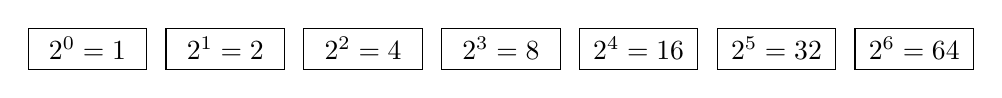
\begin{tikzpicture}[every node/.style={draw,align=center}]
  \path let \n1={width("$2^6=64$")} in foreach [count=\i, evaluate=\X as \Xeval using int(\X)] \X in {2^0,2^...,2^6} { (1.75*\i,0) node[minimum width=\n1+1em] {$\X=\Xeval$} };
\end{tikzpicture}
%% *** END OF EXAMPLE CODE ***

\end{document}
